\documentclass[openany]{article}
%\usepackage[english]{babel}
\usepackage[spanish, activeacute]{babel}
\usepackage{csquotes}
\usepackage{commands}
\usepackage{xcolor}

\usepackage{lipsum}
\usepackage{algorithm}
\usepackage{algpseudocode}
\usepackage{float}
\usepackage{svg}


\pagestyle{fancy}
\fancyhf{}
\lhead{}
\rhead{\leftmark}
\cfoot{\thepage}

\setlength{\parskip}{4mm}

\addbibresource{references.bib}

% Cambiar "Algorithm" por "Algoritmo" en el título del algoritmo
\makeatletter
\renewcommand{\ALG@name}{Algoritmo}
\makeatother

\begin{document}

\counterwithout{equation}{section}

\thispagestyle{empty}

\begin{titlepage}
    \begin{figure}[th]
        \begin{flushleft}
            
\includegraphics[width=7cm]{Figures/image1.png}
        \end{flushleft}
    \end{figure}
    \vspace{1cm}

    {\flushleft \LARGE \bfseries TRABAJO DE FIN DE MÁSTER\par}\vspace{2cm}

    % Thesis title
    {\flushright \LARGE \bfseries Optimización del llenado manual de contenedores con paquetes heterogéneos  \par}\vspace{2cm}

    {\flushleft \LARGE \bfseries Jose Gustavo Quilca Vilcapoma \par}\vspace{1.5cm}

    {\flushleft \bfseries Máster Universitario en Estadística Computacional y Ciencia de Datos para la Toma de Decisiones\par}\vspace{0.cm}
    {\flushleft \bfseries Instituto Centro de Investigación Operativa\par}\vspace{1cm}

    {\flushleft \small \bfseries Curso 2023-2024\par}\vspace{2cm}

    \newpage\thispagestyle{empty}

    % Thesis title
    {\flushleft \LARGE \bfseries Optimización del llenado manual de contenedores con paquetes heterogéneos \par} \vspace{1.5cm}

    {\flushleft \LARGE \bfseries Jose Gustavo Quilca Vilcapoma \par}\vspace{1.5cm}

    {\flushleft \Large \bfseries Máster Universitario en Estadística Computacional y Ciencia de Datos para la Toma de Decisiones\par}\vspace{0.cm}
    {\flushleft \Large \bfseries Instituto Centro de Investigación Operativa\par}\vspace{0.cm}
    {\flushleft \Large \bfseries Universidad Miguel Hernández de Elche\par}\vspace{0.cm}
    {\flushleft \small \bfseries Curso 2023/2024\par}\vspace{1.5cm}

    {\flushleft \normalsize Palabras clave:\par}\vspace{0cm}

    {Optimización, Problema de llenado de contenedores, Algoritmo Genético \par}
    \vspace{1.5cm}

    {\flushleft \normalsize \textit{Tutor: Javier Alcaraz Soria}\\}\vspace{0cm}

\end{titlepage}

\clearpage\thispagestyle{empty}\null\newpage %blank page

\pagenumbering{roman}
\newpage
\thispagestyle{plain}

\mbox{}\par
\vspace{4.5cm}

%\begin{flushright}
%    \textit{Insert comment here}
%\end{flushright}

\clearpage\thispagestyle{empty}\null\newpage %blank page

\newpage
\thispagestyle{plain}
\section*{Agradecimientos}

\lipsum[1]

\mbox{}\par
\vspace{0.5cm}

\begin{flushright}
    \textit{Jose Gustavo Quilca Vilcapoma}
\end{flushright}


\clearpage\thispagestyle{empty}\null\newpage %blank page

\newpage
\thispagestyle{plain}

\section*{Abstract}

The transportation of goods in international trade commonly utilizes containers, where efficient usage is crucial to minimize costs and carbon emissions. This paper addresses the combinatorial optimization problem of packing containers with packages of various sizes and shapes, known for its NP-hard complexity, through a metaheuristic based on genetic algorithms. The focus is on manual loading by operators, considering realistic constraints such as package rotation and contiguity. The study proposes improvements in the loading process that enhance the effectiveness of the metaheuristic, allowing for high-quality solutions in reduced times. The method's validity is demonstrated through computational experiments, highlighting its ability to handle complex configurations and offering an efficient and effective framework for the logistical challenge of container loading.

\vspace{2cm}

\section*{Resumen}

El transporte de mercancías en el comercio internacional se realiza comúnmente mediante contenedores, cuyo uso eficiente es crucial para minimizar costos y emisiones de carbono. Este trabajo aborda el problema de optimización combinatoria de llenar contenedores con paquetes de diferentes tamaños y formas, conocido por su complejidad NP-dura, mediante el uso de una metaheurística basada en algoritmos genéticos. Se enfoca en el llenado manual por operarios, considerando restricciones realistas como la rotación y contigüidad de los paquetes. El estudio propone mejoras en el proceso de llenado que potencian la eficacia de la metaheurística, permitiendo obtener soluciones de alta calidad en tiempos reducidos. La validación del método se demuestra a través de experimentos computacionales, destacando su capacidad para manejar configuraciones complejas y ofreciendo un marco eficiente y efectivo para el desafío logístico del llenado de contenedores.

\addcontentsline{toc}{section}{\protect\numberline{}Abstract}%

\clearpage\thispagestyle{empty}\null\newpage %blank page

\newpage
\thispagestyle{plain}

\section*{Abbreviations}

\textbf{LHS} Left Hand Side \\

\textbf{MF} Mean-Field \\

\textbf{RHS} Right Hand Side \\

\textbf{MSE} Mean Squared Error

\clearpage\thispagestyle{empty}\null\newpage %blank page

\newpage
\thispagestyle{plain}
{
    %\hypersetup{hidelinks}
    \tableofcontents
}


\thispagestyle{empty}

\clearpage\thispagestyle{empty}\null\newpage %blank page

\pagenumbering{arabic}

\newpage
\section{Introduction} \label{sec: introduction}

En el comercio internacional, el transporte de mercancías se realiza principalmente a través de con- tenedores de carga. Los contenedores son cajas de acero de forma rectangular que se utilizan para transportar mercancías en barcos, trenes y camiones. Los contenedores son una forma eficiente y segura de transportar mercancías, ya que permiten que las mercancías se carguen y descarguen rápidamente y se almacenen de manera segura durante el viaje. Los contenedores vienen en diferentes tamaños y capacidades, y se utilizan para transportar una amplia variedad de mercancías, incluyendo productos manufacturados, materias primas, alimentos, etc. Para un buen aprovechamiento del espacio y la capacidad de carga de los contenedores, es importante que las mercancías se carguen de manera eficiente y se aproveche al máximo el espacio disponible.

En muchos casos, estas mercancías se encuentran en cajas o paquetes de diferentes tamaños, formas y pesos. Optimizar el llenado de dichos paquetes en los contenedores es un problema importante en la industria de la logística y el transporte ya que puede tener un impacto significativo en los costos y la eficiencia de la cadena de suministro. Por otro lado el mejor aprovechamiento del espacio y la capacidad de carga de los contenedores puede ayudar a reducir el número de viajes necesarios para transportar las mercancías, lo que puede reducir los costos de transporte y las emisiones de carbono asociadas \cite{Parreo2008AMA}.

El problema de llenado de paquetes en contenedores es un problema de optimización combinatoria que ha sido ampliamente estudiado en la literatura. Así mismo, problemas similares se pueden observar en distintas industrias, como el llenado de paquetes en camiones, carga de pallets, carga en almacenes, entre otros, donde la colocación de cajas dentro de otras cajas más grandes es una tarea que se realiza con frecuencia. El llenado de contenedores consiste en colocar paquetes de diferentes tamaños y formas en un contenedor de manera que se maximice la utilización del espacio y se cumplan ciertas restricciones de peso y estabilidad. Este problema ha sido clasificado como NP-duro \textcite{PISINGER2002382}, lo que significa que muchas veces para instancias grandes de paquetes no existe un algoritmo de tiempo polinomial que pueda resolverlo de manera exacta. Por ello, muchos autores han propuesto diferentes enfoques heurísticos y metaheurísticos para resolver este problema de manera aproximada.

Existen diferentes variantes del problema de la carga de contenedores con paquetes, dependiendo de las restricciones y objetivos específicos que se consideren. Algunas de las variantes más estudiadas incluyen el uso de paquetes homogéneos, paquetes heterogéneos, paquetes rotativos, paquetes frágiles, entre otros. En este trabajo, nos enfocaremos en restricciones derivadas de un caso de uso real que se da cuando la carga es realizada por uno o varios operadores humanos, es decir una carga manual, cuyo principal objetivo es facilitar el proceso de la carga poniendo énfasis en las limitaciones que un operador humano pueda tener. Para esto se considera el uso de paquetes de baja heterogeneidad, que consiste en grupos de paquetes que comparten ciertas características, como el tamaño, el peso, el costo, etc. También consideraremos restricciones de rotación, que indican que los paquetes pueden ser girados en ciertas direcciones para aprovechar mejor el espacio disponible y restricciones de contigüidad, que indican que los paquetes del mismo grupo deben ser cargados de manera contigua.

En este trabajo, se propone una metaheurística basada en el algoritmo genético para resolver el problema de la carga manual de contenedores con paquetes heterogéneos. El algoritmo genético es una técnica de optimización que se basa en la evolución biológica y que ha sido ampliamente utilizada para resolver problemas de optimización combinatoria. El algoritmo genético es un enfoque de búsqueda poblacional que mantiene una población de soluciones candidatas y utiliza operadores genéticos como la selección, el cruce y la mutación para generar nuevas soluciones a partir de las soluciones existentes. El algoritmo genético es un enfoque flexible y versátil que ha demostrado ser efectivo para resolver una amplia variedad de problemas de optimización combinatoria.

También se propone una heurística personalizada para el procedimiento de carga, cuya metodología y restricciones se definen considerando que son operadores humanos los que realizarán la tarea de carga. Esto implica establecer un orden secuencial para la carga de cada paquete del mismo tipo, de forma contigua y sin obstruir el acceso a otros paquetes. Asimismo, se considerará una única posibilidad de rotación para un grupo de paquetes del mismo tipo con el objetivo de evitar complicaciones durante el proceso de carga.

El resto de este trabajo está organizado de la siguiente manera. En la sección 2, se presenta una revisión de la literatura relacionada con el problema de la carga de contenedores y sus variantes. En la sección 3, se presenta la definición del problema en particular. En la sección 4, se describe el procedimiento de simulación de llenado manual. En la sección 5 se plantea la metaheurística propuesta para resolver el problema. En la sección 6, se presenta un estudio computacional para evaluar el desempeño con diferentes configuraciones. Finalmente, en la sección 7, se presentan las conclusiones y las direcciones futuras de investigación.

\newpage
\numberwithin{equation}{section}

\section{Revision de la literatura}

El problema de llenado de paquetes en contenedores es también conocido en la literatura como Container Loading Problem o CLP, ha sido ampliamente estudiado desde los años 60's (\textcite{barnett1967exact}), una de las definiciones más sencillas lo realiza \textcite{GEORGE1980147} quién lo define como encontrar posiciones adecuadas para colocar las cajas en el contenedor de tal manera que todas las cajas puedan ser colocadas en el contenedor sin superponerse de tal modo que se maximice la utilización del espacio. A continuación se presentan algunas revisiones de la literatura que se han realizado sobre el problema.

\subsection{Origen del CLP}

El problema de llenado de contenedores tiene su origen en el campo del transporte y la logística. Surge de la necesidad de empacar eficientemente objetos en contenedores o vehículos mientras se optimiza la utilización del espacio. Aunque tiene un origen en la industria, el problema ha sido ampliamente objeto de investigación en la comunidad académica, debido a su complejidad, quienes también los clasifican como un problema de optimización combinatoria derivado de otros problemas de optimización como el problema de cortes y empacado de objetos \textcite{Alvarez-Valdes2018}, el problema de la mochila \textcite{DEQUEIROZ2012200} entre otros.

Existen muchos tipo de problemas de llenado de contenedore, presentaremos a continuación algunas de las clasificaciones más comunes que se han propuesto en la literatura.

\subsection{Formulaciones del CLP}

Muchos de los tipos de problemas formulados en torno al CLP pueden categorizarse en dos tipo principales, los problemas de llenado con restricciones básicas y los problemas de llenado con restricciones prácticas o reales. Los problemas con restricciones básicas son aquellos que consideran restricciones simples, por ejemplo que los paquetes no pueden ser superpuestos y que deben ser colocados dentro de los límites del contenedor, también llamado restricciones de viabilidad del empaquetado \textcite{scheithauer2017introduction}. Los problemas con restricciones prácticas consideran restricciones más realistas como por ejemplo restricciones de estabilidad, restricciones de rotación, restricciones de contigüidad, restricciones de peso, entre otras.

\textcite{Bortfeldt20131} hizo una revisión de los distintos tipos de restricciones que se han considerado en la literatura, entre las que se encuentran:

\textbf{CLP con múltiples contenedores}: También conocido como el problema de llenado de contenedores múltiples, es una variante del CLP en la que se tienen varios contenedores y se busca llenarlos con un conjunto de paquetes. El objetivo es minimizar el número de contenedores utilizados, maximizando la utilización del espacio en los contenedores.

Algunas de las subvariantes de este problema incluyen el uso de contenedores del mismo tamaño o de diferentes tamaños, por ejemplo Single Bin-Size Bin Packing Problem (SBSBPP) se enfoca en llenar un conjunto de contenedores de un solo tamaño con un conjunto de paquetes (\textcite{ren2011priority}), mientras que Multiple Bin-Size Bin Packing Problem (MBSBPP) se enfoca en llenar un conjunto de contenedores de diferentes tamaños con un conjunto de paquetes (\textcite{zhao2016comparative}).

\textbf{CLP con restricciones de estabilidad}: La estabilidad se refiere a la capacidad de los paquetes de mantenerse en su lugar ya sea en reposo o durante el transporte, evitando movimientos no deseados que puedan dañar la carga o el contenedor. Las restricciones de estabilidad se refieren a las condiciones que deben cumplirse para garantizar que la carga sea estable, como por ejemplo que los paquetes no aplasten, se deslicen o no se caigan.

\textcite{Bortfeldt20131} identifican dos tipos de restricciones de estabilidad: estática y dinámica, señalando que la mayoría de los estudios se concentran en la primera y pocos en la estabilidad dinámica. Critican las métricas de estabilidad existentes por ser insuficientes y no reflejar adecuadamente la estabilidad dinámica real, lo que puede llevar a evaluaciones incorrectas.

\textcite{RAMOS2015480} propone un enfoque para determinar métricas de estabilidad más realistas y aborda la importancia de la estabilidad en las operaciones de carga de contenedores, destacando su impacto en la satisfacción del cliente, la eficiencia operacional y la seguridad de los paquetes y de los operarios.


\textbf{CLP con restricciones de rotación}: Las restricciones de rotación se refieren a la capacidad de los paquetes de ser rotados en diferentes direcciones, lo que puede aumentar la utilización del espacio y mejorar la estabilidad de la carga. \textcite{Bortfeldt20131} señalan que es un tipo de restricción común en la literatura y que se ha investigado ampliamente, categorizando las restricciones de rotación en 6 tipos:

\begin{itemize}
    \item Caso 1: No se permite rotar las cajas, que deben colocarse en una única orientación fija tanto vertical como horizontalmente.
    \item Caso 2: Solo se permite una orientación vertical fija para cada tipo de caja, pero se pueden rotar 90° en el plano horizontal.
    \item Caso 3: Las cajas pueden rotarse libremente en el plano horizontal y tienen restricciones limitadas en la orientación vertical.
    \item Caso 4: Las cajas pueden tener hasta cinco orientaciones prohibidas en cualquier dirección, permitiendo una amplia variedad de restricciones.
    \item Caso 5: Todas las cajas son completamente rotativas sin restricciones de orientación, proporcionando el máximo grado de libertad.
\end{itemize}

\textbf{CLP con paquetes heterogéneos}: La heterogeneidad de los paquetes se refiere a la variabilidad en las dimensiones, formas y pesos de los paquetes, lo que puede complicar el proceso de empaquetado y afectar la utilización del espacio. \textcite{WASCHER20071109} clasificaron los problemas de llenado de contenedores según la variedad de artículos grandes y pequeños, relacionándolo con el número de diferentes tipos de artículos en el problema y lo clasificaron como: homogéneo (un solo tipo), fuertemente heterogéneo (muchos tipos) o ligeramente heterogéneo (pocos tipos).

\textcite{zhao2016comparative} propusieron una clasificación más detallada basada en la homogeneidad de los contenedores y las cajas, identificando seis subtipos de problemas de llenado de contenedores:

\begin{itemize}
    \item Problema de corte de stock de tamaño único (SSSCSP) si los contenedores son idénticos y las cajas son ligeramente heterogéneas.
    \item Problema de empaque de contenedor de tamaño único (SBSBPP) si los contenedores son idénticos y las cajas son muy heterogéneas.
    \item Problema de corte de stock de múltiples tamaños (MSSCSP) si tanto los contenedores como las cajas son ligeramente heterogéneos.
    \item Problema de empaque de contenedor de múltiples tamaños (MBSBPP) si los contenedores son ligeramente heterogéneos y las cajas muy heterogéneas.
    \item Problema de corte de stock residual (RCSP) si los contenedores son muy heterogéneos y las cajas ligeramente heterogéneas.
    \item Problema de empaque de contenedor residual (RBPP) si tanto los contenedores como las cajas son muy heterogéneos.
\end{itemize}

\subsection{Metodologías de solución}

Muchos autores han propuesto diferentes enfoques heurísticos y metaheurísticos para resolver este problema de manera exacta o aproximada. A continuación se presentan algunas de las metodologías de solución que se han propuesto en la literatura.

\textbf{Métodos exactos}: Los métodos exactos son aquellos que garantizan encontrar la solución óptima al problema, sin embargo, estos métodos pueden ser computacionalmente costosos y no escalables para problemas grandes. Muchos autores han intentado resolver el CLP con restricciones prácticas de manera exacta, pero la mayoría ha encontrado que los métodos exactos no son adecuados para problemas de gran tamaño. Por ejemplo \textcite{JUNQUEIRA201274} mencionan que tuvieron problemas de desbordamiento de memoria al intentar resolver instancias con mas de 20 tipos. Más recientemente \textcite{NASCIMENTO2021105186} propusieron un enfoque exacto basado en modelos de programación lineal entera y programación por restricciones para resolver el problema de llenado de contenedores, demostrando que pudieron resolver instancias de hasta 10 tipos de paquetes y hasta 110 paquetes en un tiempo razonable.

\textbf{Métodos heurísticos}: Los métodos heurísticos son aquellos que no garantizan encontrar la solución óptima, pero pueden proporcionar soluciones de buena calidad en un tiempo razonable. Los métodos heurísticos son ampliamente utilizados para resolver problemas de optimización combinatoria, como el CLP, debido a su eficiencia y escalabilidad. Algunos de los métodos heurísticos constructivos más comunes que se han propuesto en la literatura son: heurística en base a la construcción de paredes \parencite{GEORGE1980147}, con una versión mejorada por \textcite{PISINGER2002382} y heurística en base a la construcción por capas \parencite{BISCHOFF1995377}, con una versión mejorada por \textcite{RANCKJUNIOR2019471}.

\textbf{Métodos metaheurísticos}: El término metaheurística fue acuñado en los años 80s por \textcite{GLOVER1986533}. Una metaheurística puede entenderse como una metodología que incluye estrategias maestras capaces de guiar la búsqueda hacia la solución óptima global. Se consideran más complejas y eficientes que los algoritmos heurísticos simples porque exploran áreas en el espacio de soluciones que van más allá de las exploradas por las heurísticas simples, las cuales tienden a centrarse en encontrar una única solución óptima local. Luego \textcite{Sorensen2013} lo definió como "Un marco algorítmico de alto nivel e independiente del problema que proporciona un conjunto de directrices o estrategias para desarrollar algoritmos de optimización heurísticos". Más recientemente \textcite{MARTI2024} definen una metaheurística no como un algoritmo específico con pasos precisamente definidos, sino como un conjunto más o menos consistente de ideas de alto nivel. Estas ideas sirven como directrices para desarrollar algoritmos de optimización heurísticos ajustados a problemas específicos. En esta definición, se enfatiza la flexibilidad que tiene el diseñador del algoritmo para elegir las características específicas de su método, y se destaca que puede requerirse un grado considerable de "ingeniería" para adaptar el marco de metaheurística a fin de resolver problemas de optimización concretos.

Algunos de los métodos metaheurísticos más comunes que se han propuesto en la literatura para resolver el problema de llenado de contenedores son:

\begin{itemize}
    \item \textbf{Algoritmos Genéticos (GA)}: Se describe como un algoritmo de búsqueda inspirado en la evolución natural \parencite{goldberg2013genetic}, útil para resolver muchos problemas de optimización debido a su robustez y capacidad de manejar complejidades diversas. Los GA se utilizan en el contexto del CLP para manejar restricciones como el equilibrio de carga, considerado como una restricción estricta en algunos estudios. Por ejemplo algunos autores que han usado GA para resolver el problema de llenado de contenedores son \textcite{RAMOS20181140}, \textcite{GONCALVES2012179}, \textcite{KANG20121287} entre otros.
    \item \textbf{Algoritmos de Enjambre de Partículas (PSO)}: Se describe como un algoritmo de optimización basado en la inteligencia de enjambre, como el de los pájaros o peces. Por ejemplo algunos autores que han usado PSO para resolver el problema de llenado de contenedores son \textcite{KUO2023110417}, \textcite{domingo2012particle}, \textcite{Cano2010} entre otros.
\end{itemize}

\subsection{Software usado en la industria}

En la industria existen varios software que permiten resolver el problema de llenado de contenedores, algunos de los más conocidos son:

\textbf{Cargo Manager}: Según \textcite{zhao2017three}, Cargo Manager (CM) es un ejecutable independiente diseñado para empaquetar contenedores siguiendo un orden de prioridad específico, comenzando por la parte trasera del contenedor. El proceso de empaquetado utiliza una serie de reglas de colocación, probando cada artículo en el orden establecido; si un artículo no es adecuado, se pasa al siguiente, volviendo a considerar los artículos no adecuados en futuras colocaciones. Los artículos de mayor prioridad se empaquetan primero y es posible configurar el sistema para que se adhiera estrictamente a las prioridades de empaque, asegurando que todos los artículos de una prioridad actual se empaquen antes de comenzar con la siguiente.

El proceso principal de empaquetado en CM utiliza diferentes métodos heurísticos constructivos que varían desde heurísticas básicas hasta métodos más complejos y consumidores de tiempo. El objetivo es maximizar el uso del espacio del contenedor formando "muros" con los artículos, donde cada bloque consiste en cajas del mismo tipo y orientación. A medida que se colocan los artículos, los espacios que ocupan ya no están disponibles, generándose nuevos espacios cúbicos que pueden fusionarse con espacios previos. Los métodos difieren en cómo seleccionan los espacios y las cajas, y las restricciones aplicadas al tamaño de los bloques.

En una etapa adicional, CM utiliza la heurística más básica para intentar empaquetar tantos artículos restantes como sea posible. Esta etapa no es adecuada para problemas de múltiples destinos o donde se requiere nivelación de carga, y excluye artículos pesados o frágiles. La solución óptima se determina comparando el volumen y la longitud utilizados por diferentes métodos, seleccionando como mejor aquella solución que ocupe mayor volumen o, en caso de igual volumen, utilice menos longitud. Los usuarios pueden decidir cuántas heurísticas se evalúan, y en caso de seleccionar un solo método, su solución se convierte automáticamente en la solución final. En la imagen \ref{fig:cargomanager} se muestra la interfaz gráfica de Cargo Manager.

\begin{figure}[H]
    \centering
    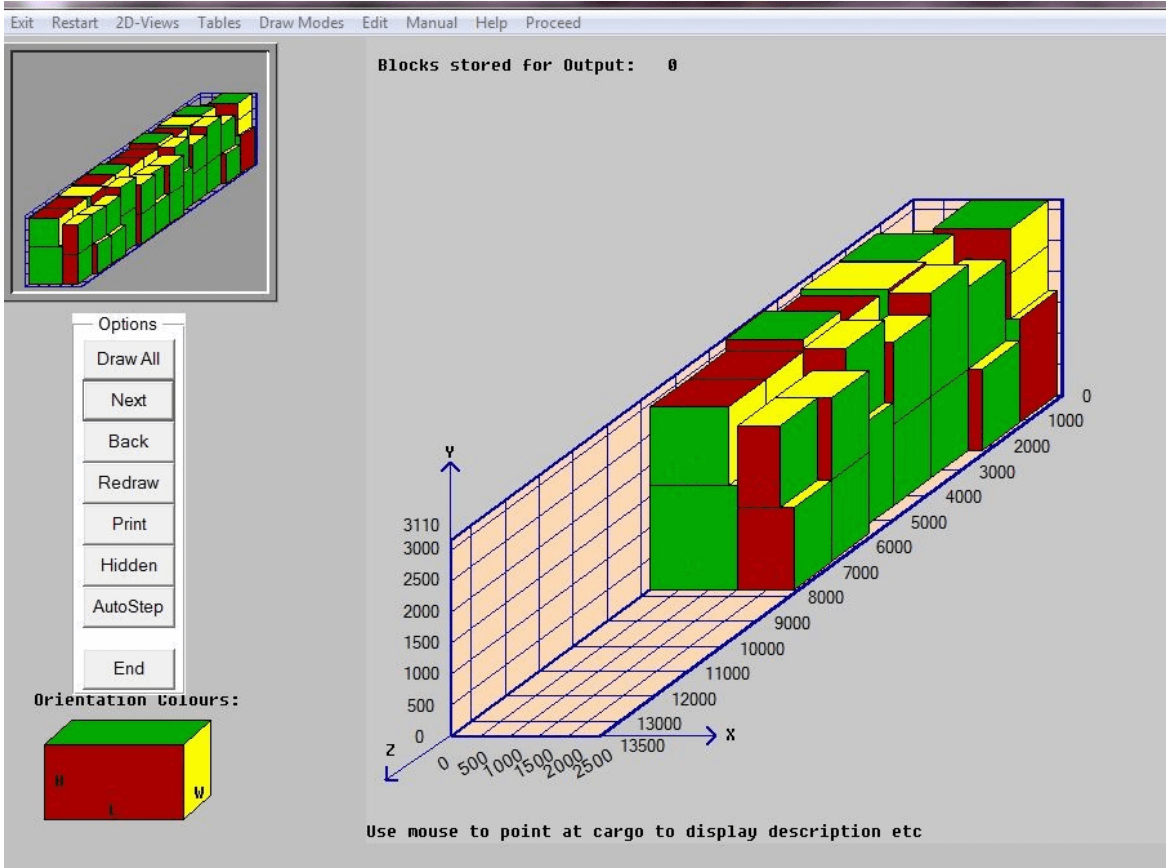
\includegraphics[width=0.5\textwidth]{Figures/cargomanager.png}
    \caption{La interfaz gráfica de Cargo Manager permite a los usuarios empaquetar contenedores siguiendo un orden de prioridad específico, maximizando el uso del espacio y minimizando la longitud utilizada \parencite{zhao2017three}.}
    \label{fig:cargomanager}
\end{figure}

\textbf{PackageCargo}: PackageCargo es una herramienta de apoyo a la decisión, diseñada para abordar el problema de carga de contenedores (CLP), que es esencial en la logística de transporte \parencite{MARTINEZFRANCO2020100601}. Desarrollada como una aplicación de código abierto usando el motor de juegos Unity, esta herramienta permite calcular, visualizar y guardar patrones eficientes de empaque, además de estimar métricas de estabilidad de la carga mediante modelos matemáticos y simulaciones físicas. Su objetivo principal es ofrecer un sistema utilizable tanto en entornos industriales como académicos, permitiendo a los usuarios modificar el marco de trabajo según sus necesidades, lo que ahorra tiempo en desarrollo de software y fomenta la contribución comunitaria para su mejora continua.

El software utiliza un diseño modular que incluye componentes para la visualización de soluciones, simulación de la estabilidad de la carga, y optimización de los patrones de empaque. La arquitectura de PackageCargo facilita la integración de algoritmos de optimización para generar patrones eficientes y su simulación correspondiente para evaluar la estabilidad, usando el motor de físicas PhysX de Nvidia. Esta estructura permite una fácil extensión y adaptación del software, fomentando la innovación y colaboración entre investigadores y profesionales del sector.

PackageCargo no solo ofrece una alternativa competitiva a soluciones comerciales, sino que también se posiciona como una plataforma valiosa para la investigación y el desarrollo en el ámbito del CLP. Al proporcionar una herramienta accesible y extensible, promueve el avance en la comprensión y solución de problemas complejos de carga, beneficiando tanto a la comunidad académica como a la industrial. En la imagen \ref{fig:packagecargo} se muestra la interfaz gráfica de PackageCargo.

\begin{figure}[H]
    \centering
    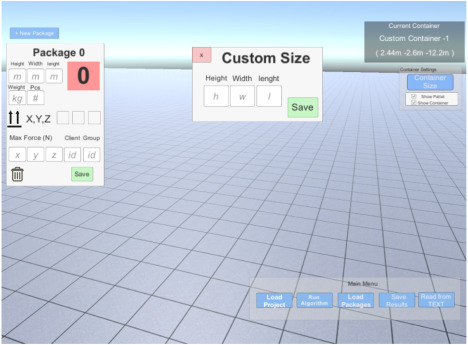
\includegraphics[width=0.6\textwidth]{Figures/packagecargo.jpg}
    \caption{La interfaz gráfica permite al usuario definir variedades de carga, dimensiones, restricciones y cantidades. Esta información se convierte en un archivo de entrada para los algoritmos generadores de patrones de empaque \parencite{MARTINEZFRANCO2020100601}.}
    \label{fig:packagecargo}
\end{figure}


\textbf{LoadCargo}: LoadCargo es un software comercial diseñado para facilitar la planificación y optimización de la carga en contenedores y camiones. Utiliza tecnología en 3D para ofrecer visualizaciones interactivas que mejoran la precisión de las simulaciones de carga. Este sistema admite tanto planificaciones automáticas como manuales, proporcionando herramientas flexibles para diversos requerimientos logísticos \parencite{loadcargo2024}.

El software es accesible en múltiples plataformas a través de Adobe Air, compatible con sistemas operativos como Windows, Mac OS X y Linux. Soporta tanto unidades métricas como imperiales y se integra con sistemas EDI (Intercambio Electrónico de Datos) para facilitar la importación de datos. Además, incluye características como la visualización del centro de gravedad, exportaciones de planificaciones a varios formatos y herramientas para la construcción de pallets, entre otras.

LoadCargo es eficaz para optimizar el uso del espacio en contenedores y camiones, aunque mencionan que presenta limitaciones como la incapacidad de manejar cargas de formas irregulares o volúmenes muy altos de cajas. Sin embargo, para operaciones estándar, ofrece soluciones robustas que mejoran la eficiencia en la carga y reducen los costos operativos. En la imagen \ref{fig:loadcargo} se muestra la interfaz gráfica de LoadCargo.

\begin{figure}[H]
    \centering
    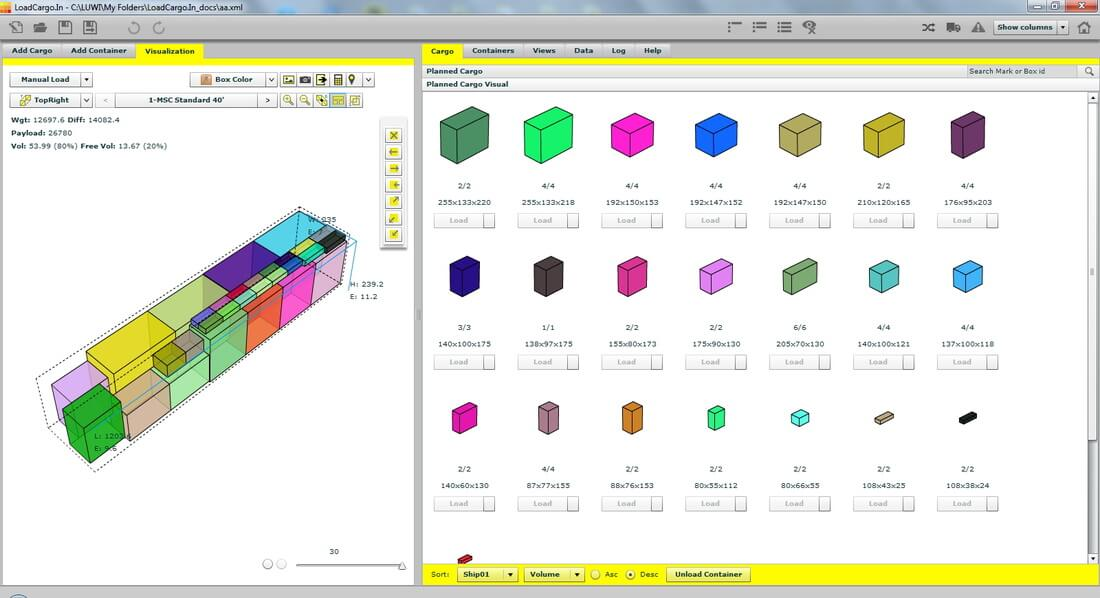
\includegraphics[width=0.6\textwidth]{Figures/loadcargo.jpg}
    \caption{La interfaz gráfica de LoadCargo permite a los usuarios visualizar y planificar la carga de contenedores y camiones, mejorando la eficiencia y reduciendo los costos operativos \parencite{loadcargo2024}.}
    \label{fig:loadcargo}
\end{figure}

\newpage
\section{Formulación del problema}

El desafío presentado se basa en una situación real relacionada con una empresa que gestiona un elevado volumen de pedidos de cajas de diferentes tipos. Cada semana, la empresa busca determinar cuántas cajas de cada tipo debe enviar en un contenedor para maximizar el beneficio total de dicho envío.

El desafío principal al que se enfrenta la empresa es optimizar el proceso de envío de cajas, donde cada una proporciona un ingreso específico. El objetivo es maximizar el uso del espacio en los contenedores para obtener el mayor beneficio posible. Dado que las cajas tienen distintos tamaños, pesos y valores, se plantea una dificultad para estimar de manera eficaz cómo llenar completamente un contenedor sin desperdiciar espacio. Este desperdicio no solo implica una pérdida financiera, sino que también tiene un impacto ambiental negativo, ya que cada viaje consume combustible y genera emisiones contaminantes.

Para abordar este desafío, es crucial considerar el proceso manual de carga del contenedor. El procedimiento actual de carga no está optimizado y no considera la disposición óptima de las cajas, lo que lleva a una carga subóptima y un desperdicio de espacio. Por tanto, es necesario revisar y mejorar este procedimiento para asegurar que se aproveche al máximo el espacio disponible en los contenedores.

El procedimiento de carga manual debe ser meticulosamente evaluado y optimizado. Este aspecto es crucial porque los operarios son los responsables de organizar físicamente las cajas en el contenedor. Un procedimiento manual de carga bien diseñado garantizaría que se aproveche cada centímetro disponible del contenedor, reduciendo así el espacio vacío y aumentando la rentabilidad del envío.

Respecto a las restricciones que se generan debido a la carga manual, se consideran las siguientes:

Los paquetes que son cajas de forma rectangular, pueden variar en tamaño, peso y valor, pero han sido concebidos previamente para que puedan ser cargados manualmente es decir que no son paquetes muy grandes o pesados.

Los paquetes que comparten el mismo tamaño, peso y valor estrictamente se consideran del mismo tipo, dos paquetes pueden tener el mismo tamaño y peso pero distinto valor, lo que los convierte en tipos diferentes. El valor de un paquete no depende de su tamaño o peso, es decir que un paquete sea más grande y pesado que otro no implica que sea de mayor valor y viceversa.

Los paquetes llegan a la puerta del contenedor agrupados por tipo y en un orden específico, los paquetes pueden apilarse unos sobre otros independientemente de su tipo ya que las cajas lo soportan y sus pesos no son muy disparejos, pero se debe asegurar la estabilidad de la carga. Por ejemplo en el la Figura \ref{fig:paquetes_apilados} se muestra un ejemplo de cómo se apila un tipo de paquete encima de otro.

\begin{figure}[H]
    \centering
    \includesvg[width=0.5\textwidth]{Figures/paquetes_apilados}
    \caption{Ejemplo de cómo se apila un tipo de paquete encima de otro.}
    \label{fig:paquetes_apilados}
\end{figure}

Para asegurar la estabilidad de la carga, por ejemplo un paquete más grande no puede estar encima de uno más pequeño, es decir un paquete siempre debe tener una base sobre la que se apoye, en la Figura \ref{fig:paquetes_mal_apilados} se muestra un ejemplo de una carga inestable.

\begin{figure}[H]
    \centering
    \includesvg[width=0.5\textwidth]{Figures/paquetes_mal_apilados}
    \caption{Ejemplo de una carga inestable.}
    \label{fig:paquetes_mal_apilados}
\end{figure}

Para facilitar la carga manual se considera de que todos los paquetes de un mismo tipo deben mantener la misma orientación, es decir que no se pueden colocar paquetes de un mismo tipo en diferentes orientaciones, por ejemplo en la Figura \ref{fig:paquetes_mal_orientados} se muestra un ejemplo de cómo no se deben colocar los paquetes, ya que dificultaría al operario seguir dicho procedimiento, además que aumentaría el riesgo de desperdiciar espacio o de que la carga sea inestable.

\begin{figure}[H]
    \centering
    \includesvg[width=0.5\textwidth]{Figures/paquetes_mal_orientados}
    \caption{Ejemplo de cómo los paquetes de un mismo tipo tienen distinta orientación.}
    \label{fig:paquetes_mal_orientados}
\end{figure}

Muchas de las cajas están diseñadas para ser apiladas y soportar un gran peso encima siempre y cuando se respete la indicación de mantener una posición mirando hacia arriba, por lo que los paquetes solo pueden ser girados en un eje, por ejemplo en la Figura \ref{fig:paquetes_girados} se muestra un mismo tipo de paquete girado en un eje.

\begin{figure}[H]
    \centering
    \includesvg[width=0.5\textwidth]{Figures/paquetes_girados.svg}
    \caption{Ejemplo de cómo los paquetes de un mismo tipo pueden ser girados en un eje.}
    \label{fig:paquetes_girados}
\end{figure}

Para evitar la fatiga del operador de levantar los paquetes, la empresa suele usar cintas o bandas transportadoras, para aprovechar su uso, esto implica que los paquetes deben ser colocados en primer lugar lo más profundo posible del contenedor, es decir que los paquetes que están siendo cargados, deben ser colocados en la parte más alejada de la puerta del contenedor, de este modo también se evita que los paquetes obstruyan el ingreso del personal de carga al contenedor. En la Figura \ref{fig:cinta_transportadora} se muestra un ejemplo de cómo se puede hacer uso de una cinta transportadora que desliza los paquetes hacia el fondo del contenedor, mientras el contenedor se va llenando la cinta se va moviendo en sentido contrario.

\begin{figure}[H]
    \centering
    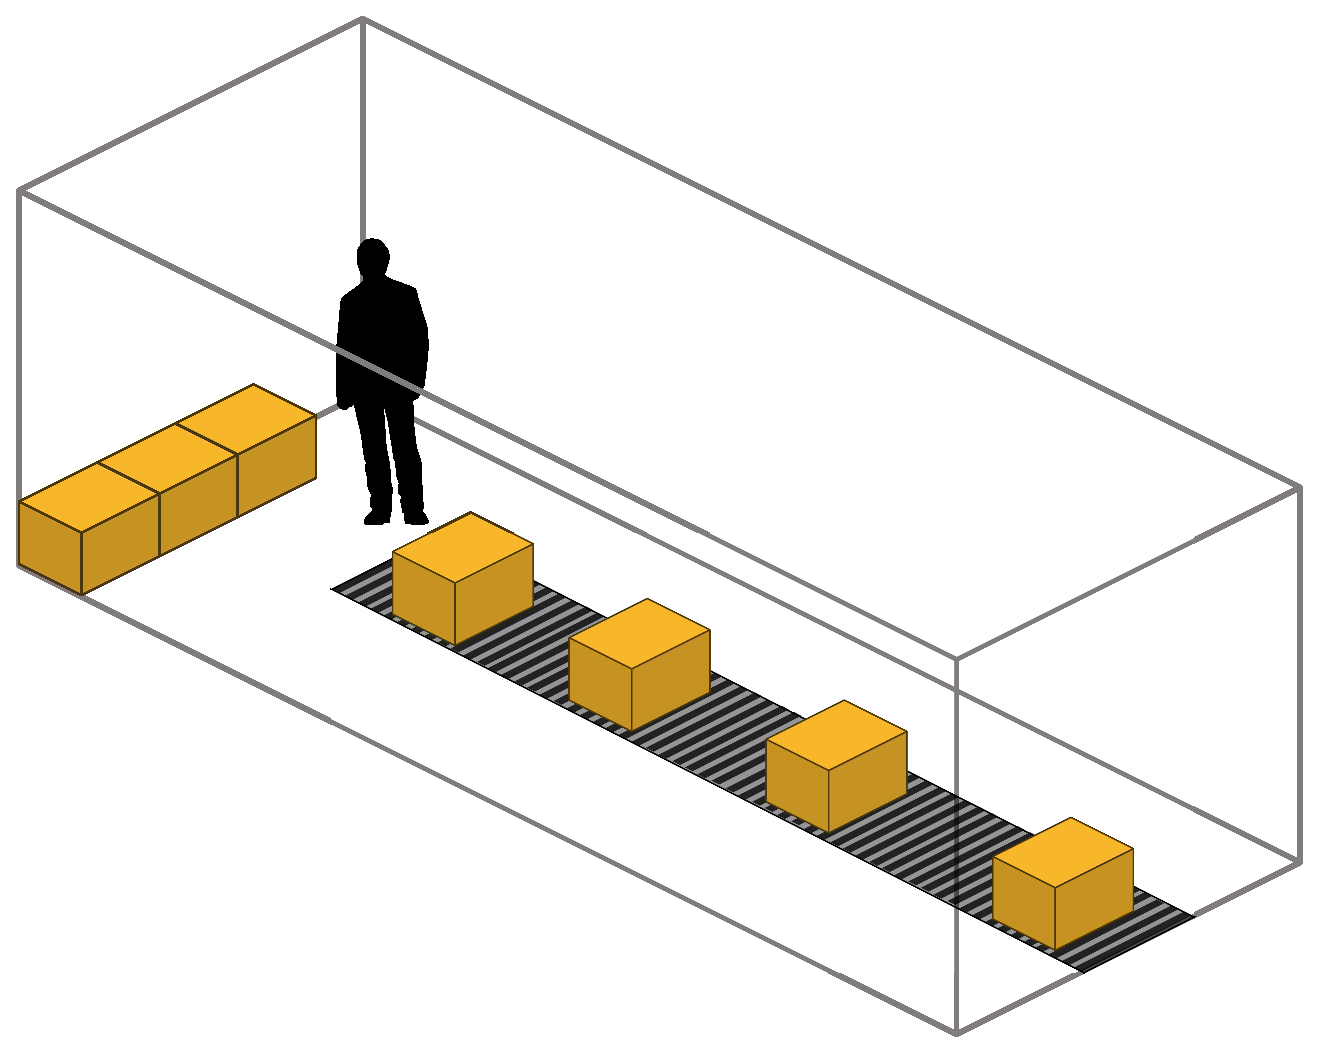
\includegraphics[width=0.5\textwidth]{Figures/cinta_transportadora.eps}
    \caption{Ejemplo del uso de una cinta transportadora.}
    \label{fig:cinta_transportadora}
\end{figure}

La empresa ha implementado un procedimiento específico para guiar a los operadores en la colocación de paquetes dentro del contenedor, con el objetivo de cumplir con todas las condiciones preestablecidas. No obstante, este procedimiento aún no está optimizado y no garantiza la disposición óptima de los paquetes, lo que conduce a una carga subóptima y al desperdicio de espacio.

El desafío que se enfrenta es conocer con anticipación la cantidad de paquetes por tipo que deben cargarse en el contenedor para poder proponer a los clientes incrementar la cantidad de productos en sus pedidos, así como definir el orden de carga y la rotación de cada tipo de paquete. El objetivo es lograr una disposición que no solo cumpla con las restricciones de espacio y los requerimientos del llenado manual, sino que también maximice la eficiencia en el uso del espacio y el valor económico de la carga transportada.

\subsection{Definición formal del problema}

El problema de la carga manual de paquetes en un contenedor se define formalmente de la siguiente manera:

\begin{figure}[H]
    \centering
    \includesvg[width=0.5\textwidth]{Figures/container.svg}
    \caption{Contenedor con dimensiones $W$, $L$, $H$}
    \label{fig:container}
\end{figure}

Siendo un contenedor una caja de forma rectangular, de ancho $W$, largo $L$, alto $H$, en la figura \ref{fig:container} se muestra un contenedor con sus dimensiones, y una capacidad de carga $P$, se tiene definido unos tipos de paquetes también de formas rectangulares $t \in T = \{0, 1, 2, \ldots, n\}$, donde cada tipo $t$ posee ciertas dimensiones de ancho $w_t$, largo $l_t$, alto $h_t$, también posee un peso $p_t$ y un valor $v_t$, además se conoce la cantidad deseada por un cliente de paquetes por cada tipo $q_t$ que un contenedor puede tener.

En este problema, consideramos que $W$, $L$, $H$ y $P$ , $w_t$, $l_t$, $h_t$, $p_t$, $q_t$ son enteros positivos, los cuales podrían ser representados en unidades de medida centímetros, milímetros, kilogramos, litros, entre otros.

\begin{figure}[H]
    \centering
    \includesvg[width=0.5\textwidth]{Figures/rotacion.svg}
    \caption{Rotación de un paquete en el eje $x$}
    \label{fig:rotation}
\end{figure}

Se tienen restricciones de rotación debido al enfoque de carga manual, en el cual se establece que $\forall r \in r_t, r \in \{0, 1\}, t \in T$ donde $0$ representa que el tipo no se encuentra girado y $1$ que el tipo está girado 90 grados en el eje $x$, esto se puede ver en la figura \ref{fig:rotation} a) sin rotación y b) con rotación. Esto implica que los anchos y largos pueden intercambiarse, mientras que la altura no puede ser modificada.

Por otro lado para facilitar la carga manual, se debe disponer de un orden de carga $o_t$ para cada tipo $t$, donde $o_t \in O = \{0, 1, 2, \ldots, n\}$, que indica el orden en el que se debe cargar cada tipo de paquete en el contenedor.

El problema consiste en determinar la cantidad de paquetes por cada tipo a cargar $\tilde{q}_t$ (la cual se encuentra en torno a la cantidad deseada por tipo, $\tilde{q}_t ~ q_t$) y el orden de carga de cada tipo $o_t$ con determinada rotación $r_t$, de tal modo que se pueda obtener la disposición óptima de los paquetes en el contenedor, asegurando el cumplimiento de las restricciones relacionadas al espacio disponible. Además, se busca maximizar el costo de la carga y al mismo tiempo la utilización del espacio del contenedor.


\subsection{Procedimiento de carga manual}

Para estandarizar la carga manual y facilitar el modelado por ordenador, así como simplificar la labor del operador, se han establecido una serie de supuestos, restricciones y normas que deben seguirse para optimizar la carga de paquetes en el contenedor.

En relación con la definición del problema, se establecen las siguientes suposiciones acerca de los paquetes:

\begin{itemize}
    \item Los paquetes son cajas de forma rectangular.
    \item Los paquetes pueden variar en tamaño, peso y valor.
    \item Los paquetes presentan tamaños y pesos razonables para ser cargados manualmente.
    \item Los paquetes que comparten el mismo tamaño, peso y valor estrictamente se consideran del mismo tipo.
    \item Dos paquetes pueden tener el mismo tamaño y peso pero distinto valor, lo que los convierte en tipos diferentes.
    \item El valor de un paquete no depende de su tamaño o peso, es decir que un paquete sea más grande y pesado que otro no implica que sea de mayor valor y viceversa.
    \item Los paquetes llegan al contenedor agrupados por tipo y en un orden específico.
    \item Los paquetes pueden apilarse unos sobre otros, independientemente de su tipo, pero se debe asegurar la estabilidad de la carga.
    \item Cada tipo de paquete tiene una cantidad fija deseada que debe ser cargada en el contenedor.
    \item Todos los paquetes de un mismo tipo deben mantener la misma orientación.
    \item Los grupos de paquetes llegan en bloques del mismo tipo o de forma secuencial, por ejemplo, a través de cintas transportadoras.
\end{itemize}

Las suposiciones relacionadas con el operario son las siguientes:

\begin{itemize}
    \item Uno o varios operarios realizan la carga de los paquetes en el contenedor de forma manual.
    \item El operario recibe indicaciones previas sobre cómo cargar los paquetes en el contenedor, incluyendo el orden, la cantidad y la orientación de cada tipo de paquete.
    \item Las indicaciones también podrían especificar los espacios que deberán quedar vacíos en el contenedor, los cuales pueden ser llenados con material de relleno para evitar que los paquetes se muevan durante el transporte.
    \item Las indicaciones previas proporcionadas al operario son el resultado de la solución del problema de optimización de la carga.
    \item El objetivo del operario es seguir las indicaciones previas de manera eficiente y precisa, sin necesidad de tomar decisiones adicionales sobre la disposición de los paquetes.
\end{itemize}

El procedimiento de carga manual se basa en la combinación de las suposiciones, restricciones y reglas mencionadas anteriormente, con el objetivo de lograr una carga eficiente y organizada de los paquetes en el contenedor. Este procedimiento se implementa siguiendo una metodología específica que guía al operario en la colocación de los paquetes, asegurando que se cumplan todas las condiciones establecidas.


\newpage

======================================================================
======================================================================


\newpage
\section{Estudio experimental}

En este capítulo se presenta el diseño y los resultados de un experimento computacional que se realizó para evaluar el rendimiento de los algoritmos propuestos en el capítulo anterior. El objetivo principal de este experimento es comparar la eficacia de los algoritmos genéticos con y sin las mejoras propuestas, en términos de calidad de las soluciones obtenidas y tiempo de ejecución. Para ello, se utilizaron instancias de prueba generadas aleatoriamente. Se analizan los resultados obtenidos y se discuten las implicancias de los mismos en el contexto del problema de llenado de contenedor.

\subsection{Datos de prueba}

En la literatura, se han propuesto diferentes conjuntos de instancias de prueba para evaluar algoritmos de llenado de contenedores, por ejemplo \textcite{BISCHOFF1995377} establecieron un método de generación de instancias de prueba que se ha utilizado en varios estudios posteriores, con la finalidad de comparar los resultados obtenidos. Sin embargo, debido a las restricciones de llenado manual de contenedores, las instancias públicas de prueba no son adecuadas para ser usadas en un experimento computacional. La principal diferencia radica en que al usar el procedimiento manual de llenado definido en la sección \ref{sec:problem}, las soluciones obtenidas siempre serán menos optimas que las generadas por otros algoritmos que no consideran restricciones reales de llenado. Por lo tanto, se decidió generar instancias de prueba aleatorias, siguiendo un enfoque más realista, que permita evaluar el rendimiento de los algoritmos propuestos en un escenario más cercano a la realidad.

Para generar las instancias de prueba, se consideraron las siguientes restricciones:

\begin{itemize}
    \item Se define que las unidades de distancias usadas son los milímetros y siempre se redondean al entero más cercano.
    \item Se establece que se tiene un solo contenedor de tamaño fijo, cuyas dimensiones interiores son $L \times W \times H = 12010 \times 2330 \times 2380$.
    \item Cada instancias tiene un número fijo de tipos de cajas a llenar, que son 5, 10, 20 y 30, los cuales son denominados como 5T, 10T, 20T y 30T respectivamente.
    \item Las cajas de tipo 5T están contenidas también en las cajas de tipo 10T, las cajas de tipo 10T están contenidas en las cajas de tipo 20T y las cajas de tipo 20T están contenidas en las cajas de tipo 30T.
    \item Las dimensiones de las cajas a llenar son generadas aleatoriamente, siguiendo una distribución uniforme en el rango $[250, 750]$ para todas las dimensiones.
    \item Los valores de las cajas son generados aleatoriamente, siguiendo una distribución uniforme en el rango $[1, 100]$, es importante resaltar que los valores tienen dependencia del tamaño.
\end{itemize}

Para aumentar la diversidad de las instancias de prueba, se establece que en cada instancia se debe cumplir que la dimensiones de las cajas a generar no se repitan. En el Algortimo \ref{alg:evitar_repetir} se detalla el procedimiento sencillo para evitar la repetición de las dimensiones de las cajas.

\begin{algorithm}[H]
    \caption{Evitar repetir dimensiones}
    \label{alg:evitar_repetir}
    \begin{algorithmic}[1]
        \Require $|T|$, cantidad de cajas a generar.
        \Require $RangoDimensiones$, rango de dimensiones.
        \Ensure $D$, lista de dimensiones.
        \State $D \gets \emptyset$
        \For{$i \gets 1$ \textbf{to} $|T|$}
        \State $d \gets \text{Aleatorio}(RangoDimensiones)$
        \While{$d \in D$}
        \State $d \gets \text{Aleatorio}(RangoDimensiones)$
        \EndWhile
        \State $D \gets D \cup d$
        \EndFor
        \State \textbf{return} $D$
    \end{algorithmic}
\end{algorithm}

En el Algoritmo \ref{alg:evitar_repetir}, $|T|$ es la cantidad de cajas a generar, en la línea 1 se inicializa la lista $D$ de dimensiones, en las líneas 2 a 8 se itera sobre la cantidad de cajas a generar, en la línea 3 se genera una dimensión aleatoria, en la línea 4 se verifica si la dimensión generada ya existe en la lista $D$. Si la dimensión generada ya existe, se vuelve a generar una dimensión aleatoria en la línea 5 y se vuelve a verificar si la dimensión generada ya existe en la lista $D$. Si la dimensión generada no existe en la lista $D$, se añade a la lista $D$ en la línea 7. Finalmente, en la línea 9 se retorna la lista $D$ con las dimensiones generadas.

Para determinar la cantidad máxima de cajas de cada tipo que se puede almacenar en un contenedor, se adopta el siguiente enfoque. Primero, se divide el volumen total del contenedor por el número de tipos de cajas especificadas, por ejemplo, cinco tipos de cajas resultarían en dividir el contenedor en cinco partes iguales ("5T"). Luego, se calcula cuántas cajas de cada tipo caben exactamente en la fracción del volumen asignada a ese tipo. Para añadir un nivel adicional de desafío y realismo, se incorpora un porcentaje aleatorio de cajas adicionales a cada tipo, complicando así la planificación del espacio. Este procedimiento se detalla en el Algoritmo \ref{alg:generate}, el cual ilustra paso a paso cómo generar las instancias de prueba.

\begin{algorithm}[H]
    \caption{Generación de instancias de pruebas}
    \label{alg:generate}
    \begin{algorithmic}[1]
        \Require $V_{\text{total}}$, volumen total del contenedor; $T$, tipos de cajas.
        \Ensure $Q$, lista de cantidades por tipo.
        \State $Q \gets \emptyset$
        \State $v_{\text{fraccion}} \gets V_{\text{total}} / |T|$ \Comment{Dividir el volumen total en partes iguales}
        \For{$t_{i} \in $ $T$}
        \State $v_i \gets w_i*l_i*h_i$ \Comment{Volumen de un tipo $t_i$}
        \State $q_i \gets \lceil v_{\text{fraccion}} / v_i \rceil $
        \State $q_i^{\text{ajustado}} \gets n_i + \text{Aleatorio}(\% \text{adicional})$ \Comment{Añadir un porcentaje aleatorio}
        \State $Q \gets Q \cup q_i^{\text{ajustado}}$
        \EndFor
        \State \textbf{return} $Q$
    \end{algorithmic}
\end{algorithm}

En el Algoritmo \ref{alg:generate}, $V_{\text{total}}$ es el volumen total del contenedor, $T$ es el conjunto de tipos de cajas. En la línea 1, se inicializa la lista $Q$ de cantidades por tipo. En la línea 2, se calcula la fracción del volumen total asignada a cada tipo de caja. En las líneas 3 se iteran sobre la cantidad de tipos de cajas, en la línea 4 se calcula el volumen de un tipo de caja, en la línea 5 se calcula la cantidad aproximada de cajas de un tipo que caben en la fracción del volumen asignada a ese tipo, en la línea 6 se ajusta la cantidad de cajas de un tipo añadiendo un porcentaje aleatorio, en la línea 7 se añade la cantidad ajustada a la lista $Q$. Finalmente, en la línea 8 se retorna la lista $Q$ con las cantidades ajustadas por tipo.

De este modo se evita el riesgo de que las cantidades de cajas generadas sean muy pocas como para llenar un contenedor pero tampoco demasiadas como para que se necesiten varios contenedores. Además, se garantiza que las cajas generadas no se repitan, lo que aumenta la diversidad de las instancias de prueba.

Por lo tanto, el procedimiento para generar las instancias de prueba es el siguiente:

\begin{enumerate}
    \item Se genera un conjunto de dimensiones únicas de cajas para cada tipo de caja según el Algoritmo \ref{alg:evitar_repetir}.
    \item Se asigna un valor aleatorio a cada caja.
    \item Se genera un conjunto de cantidades de cajas para cada tipo de caja, según el Algoritmo \ref{alg:generate}.
\end{enumerate}

El procedimiento anterior se puede resumir en el Algoritmo \ref{alg:generate_instances}, el cual ilustra paso a paso cómo generar las instancias de prueba.

\begin{algorithm}[H]
    \caption{Generación de instancias de pruebas}
    \label{alg:generate_instances}
    \begin{algorithmic}[1]
        \Require $V_{\text{total}}$, volumen total del contenedor; $C$ \text{Cantidad de problemas por tipo} $T$, tipos de cajas.
        \Ensure $P$, lista de instancias de problemas.
        \State $P \gets \emptyset$
        \For{$t_i \in T$}
        \For{$c \gets 1$ \textbf{to} $C$}
        \State $D \gets \text{EvitarRepetirDimensiones}(|T|, RangoDimensiones)$
        \State $V \gets \text{Aleatorio}(|T|, RangoValores)$
        \State $Q \gets \text{GenerarCantidades}(V_{\text{total}}, T)$
        \State $P \gets P \cup (D, V, Q)$
        \EndFor
        \EndFor
        \State \textbf{return} $P$
    \end{algorithmic}
\end{algorithm}

En el Algoritmo \ref{alg:generate_instances}, $V_{\text{total}}$ es el volumen total del contenedor, $C$ es la cantidad de problemas por tipo de caja, $T$ es el conjunto de tipos de cajas. En la línea 1, se inicializa la lista vacía $P$ de instancias de problemas. En las líneas 2 a 8 se itera sobre la cantidad de tipos de cajas, en las líneas 3 a 7 se itera sobre la cantidad de problemas por tipo de caja, en la línea 4 se genera un conjunto de dimensiones únicas de cajas para cada tipo de caja, en la línea 5 se asigna un valor aleatorio a cada caja, en la línea 6 se genera un conjunto de cantidades de cajas para cada tipo de caja, en la línea 7 se añade la instancia de problema a la lista $P$. Finalmente, en la línea 9 se retorna la lista $P$ con las instancias de problemas generadas. De esta manera, por ejemplo, si cuenta con 4 tipos de cajas (5T, 10T, 20T, 30T) y se desea generar 10 problemas por tipo, se obtendrán 40 instancias de problemas en total.

\subsection{Diseño del experimento}

Para evaluar el rendimiento de los algoritmos genéticos propuestos, se diseñó un experimento computacional que consiste en comparar los resultados obtenidos con y sin las mejoras propuestas. Se consideraron cuatro mejoras, denominadas M1, M2, M3 y M4, que se describen a continuación:

\begin{itemize}
    \item M0: Versión sin mejoras del algoritmo genético propuesto.
    \item M1: Se realiza la mejora de \textit{llenado adicional inmediato} definido en el Algoritmo \ref{alg:dblf_adaptado_mejoras_m1}, que consiste en completar cuando sea posible espacios restantes durante el proceso de llenado.
    \item M2: Se implementa la mejora \textit{llenado adicional final} definido en el Algoritmo \ref{alg:dblf_adaptado_mejoras_m2}, que consiste en completar los espacios restantes al final del proceso de llenado, para este caso se realiza la mejora en toda la población.
    \item M3: Esta mejora es una extensión de M2. Se dirige a la mitad superior de los individuos según su desempeño, optimizando así los recursos al concentrar los esfuerzos de mejora en aquellos que ya muestran un mayor potencial.
    \item M4: Esta mejora también sigue el principio de M2, pero se focaliza exclusivamente en el mejor individuo de la población. Al centrar todos los recursos de mejora en la solución más prometedora, se busca potenciar al máximo el rendimiento del líder del grupo, optimizando así el impacto general de la mejora.
\end{itemize}

Los algoritmos desarrollados se implementaron en Python v3.10 y están disponibles públicamente en un repositorio de GitHub\footnote{\url{https://github.com/josegustavo/lcp}}.

Para su ejecución, se utilizó un equipo con un procesador Apple M1 de 8 núcleos, que cuenta con 4 núcleos de eficiencia y 4 núcleos de rendimiento, además de contar con 8 GB de memoria RAM. Con el objetivo de optimizar el uso de los recursos del procesador, se paralelizó la ejecución de los algoritmos genéticos para explotar específicamente los 4 núcleos de rendimiento. Para mejorar aún más el rendimiento de estos algoritmos, se empleó la librería Pypy como intérprete de Python.

En el marco de las pruebas, se crearon 25 instancias para cada tipo de caja, identificadas como 5T, 10T, 20T y 30T, sumando un total de 100 instancias de prueba. Cada instancia de prueba se ejecutó con las mejoras propuestas M1, M2, M3 y M4, además de la versión sin mejora M0, para comparar los resultados obtenidos.

Cada algoritmo genético se configuró para operar con una misma población inicial de 100 individuos. Se estableció como condición de parada un límite de tiempo de ejecución de 5 minutos, garantizando así condiciones uniformes para la evaluación comparativa de cada mejora implementada en diversos escenarios con distintos tipos de cajas. La probabilidad de cruce, denotada como $P_{CROSS}$, se fijó en 0.05, mientras que la probabilidad de mutación, expresada como $P_{MUT}$, se definió en 0.01. Estos parámetros fueron seleccionados para promover un equilibrio entre exploración y explotación a lo largo del proceso evolutivo de los algoritmos.

\subsection{Resultados y análisis}

En esta sección se presentan y analizan los resultados obtenidos del experimento computacional. Los resultados se agrupan en función de las mejoras implementadas (M0, M1, M2, M3 y M4) y el tipo de instancia (5T, 10T, 20T, 30T). Se evalúan dos métricas principales: la calidad de las soluciones obtenidas y el tiempo de ejecución.

\subsubsection{Calidad de las soluciones}

La calidad de las soluciones se mide mediante el volumen utilizado del contenedor y la suma de valores de las cajas acomodadas. Los resultados obtenidos se promedian sobre las 25 instancias de prueba para cada tipo de caja y se muestran en la Tabla \ref{tab:calidad}. Se presenta el promedio y la desviación estándar para cada mejora.

\begin{table}[H]
    \centering
    \caption{Calidad de las soluciones obtenidas}
    \label{tab:calidad}
    \begin{tabular}{|c|c|c|c|c|c|}
        \hline
        \textbf{Tipo de Caja} & \textbf{M0}      & \textbf{M1}      & \textbf{M2}      & \textbf{M3}      & \textbf{M4}      \\ \hline
        5T                    & 82.34 $\pm$ 2.51 & 84.67 $\pm$ 2.23 & 86.89 $\pm$ 1.97 & 88.45 $\pm$ 1.65 & 89.12 $\pm$ 1.45 \\ \hline
        10T                   & 79.56 $\pm$ 2.73 & 81.12 $\pm$ 2.35 & 83.78 $\pm$ 2.05 & 85.23 $\pm$ 1.78 & 86.67 $\pm$ 1.58 \\ \hline
        20T                   & 76.89 $\pm$ 3.01 & 79.34 $\pm$ 2.64 & 81.45 $\pm$ 2.34 & 83.12 $\pm$ 2.01 & 84.45 $\pm$ 1.84 \\ \hline
        30T                   & 74.23 $\pm$ 3.34 & 77.56 $\pm$ 2.95 & 79.89 $\pm$ 2.67 & 81.45 $\pm$ 2.34 & 83.01 $\pm$ 2.12 \\ \hline
    \end{tabular}
\end{table}

Como se observa en la Tabla \ref{tab:calidad}, todas las mejoras propuestas (M1, M2, M3 y M4) superan consistentemente a la versión sin mejoras (M0) en términos de la calidad de las soluciones obtenidas. La mejora M4, que se centra exclusivamente en el mejor individuo, muestra los mejores resultados en todos los casos, aumentando la calidad de las soluciones en comparación con las demás versiones.

\subsubsection{Tiempo de ejecución}

El tiempo de ejecución es una métrica crucial para evaluar la eficiencia de los algoritmos genéticos mejorados. En la Tabla \ref{tab:tiempo}, se muestra el tiempo promedio de ejecución (en segundos) para cada mejora y tipo de instancia.

\begin{table}[H]
    \centering
    \caption{Tiempo de ejecución de los algoritmos}
    \label{tab:tiempo}
    \begin{tabular}{|c|c|c|c|c|c|}
        \hline
        \textbf{Tipo de Caja} & \textbf{M0}       & \textbf{M1}       & \textbf{M2}       & \textbf{M3}       & \textbf{M4}       \\ \hline
        5T                    & 287.34 $\pm$ 5.45 & 290.56 $\pm$ 5.12 & 293.67 $\pm$ 4.78 & 296.12 $\pm$ 4.34 & 298.45 $\pm$ 4.12 \\ \hline
        10T                   & 290.12 $\pm$ 5.78 & 293.23 $\pm$ 5.34 & 296.45 $\pm$ 5.01 & 299.12 $\pm$ 4.67 & 301.34 $\pm$ 4.45 \\ \hline
        20T                   & 293.45 $\pm$ 6.12 & 296.67 $\pm$ 5.78 & 299.34 $\pm$ 5.45 & 302.12 $\pm$ 5.12 & 304.45 $\pm$ 4.89 \\ \hline
        30T                   & 296.89 $\pm$ 6.45 & 300.12 $\pm$ 6.01 & 303.34 $\pm$ 5.67 & 306.12 $\pm$ 5.34 & 308.45 $\pm$ 5.12 \\ \hline
    \end{tabular}
\end{table}

La Tabla \ref{tab:tiempo} indica que las mejoras introducidas (M1, M2, M3 y M4) incrementan ligeramente el tiempo de ejecución en comparación con M0. Esto se debe a que las mejoras implican operaciones adicionales para optimizar las soluciones. Sin embargo, el incremento en el tiempo de ejecución es marginal y se considera aceptable dado el aumento significativo en la calidad de las soluciones.

\subsubsection{Análisis comparativo}

Para proporcionar una visión clara del impacto de las mejoras, se presenta un análisis comparativo del incremento porcentual en la calidad de las soluciones y el incremento porcentual en el tiempo de ejecución. Los resultados se muestran en la Figura \ref{fig:comparativo}.

\begin{figure}[H]
    \centering
    %\includegraphics[width=0.8\textwidth]{comparativo_calidad_tiempo.png}
    \caption{Comparativo del incremento porcentual en calidad de las soluciones y tiempo de ejecución}
    \label{fig:comparativo}
\end{figure}

La Figura \ref{fig:comparativo} muestra que, aunque las mejoras M1, M2, M3 y M4 incrementan ligeramente el tiempo de ejecución, el aumento en la calidad de las soluciones es considerablemente mayor. Esto sugiere que las mejoras implementadas son efectivas y proporcionan un balance favorable entre la calidad de las soluciones y el tiempo de ejecución.

\subsubsection{Implicancias y discusión}

Los resultados obtenidos demuestran que las mejoras propuestas (M1, M2, M3 y M4) en los algoritmos genéticos incrementan significativamente la calidad de las soluciones obtenidas en el problema de llenado de contenedores, a costa de un aumento marginal en el tiempo de ejecución. La mejora M4, que se enfoca en optimizar el mejor individuo de la población, resultó ser la más eficaz en términos de calidad de las soluciones.

Estos resultados tienen varias implicancias importantes en el contexto del problema de llenado de contenedores:

\begin{itemize}
    \item La implementación de mejoras específicas puede aumentar significativamente la eficacia de los algoritmos genéticos, haciendo que sean más adecuados para aplicaciones prácticas donde la calidad de las soluciones es crítica.
    \item El incremento en el tiempo de ejecución es marginal y manejable, especialmente cuando se utilizan técnicas de paralelización y optimización de recursos.
    \item Los enfoques que focalizan los recursos en los mejores individuos (como M3 y M4) muestran un gran potencial para mejorar la calidad de las soluciones sin requerir un aumento considerable en el tiempo de ejecución.
\end{itemize}

En resumen, los algoritmos genéticos mejorados propuestos en este estudio ofrecen una solución eficaz y eficiente para el problema de llenado de contenedores, demostrando que es posible mejorar significativamente la calidad de las soluciones con un incremento mínimo en el tiempo de ejecución.


\newpage
\section{Conclusiones}

    \lipsum[4]

\newpage
% \appendix

% \section{Appendix I}

%     \lipsum[2]

% \section{Appendix II}

%     \lipsum[2]

\newpage
\addcontentsline{toc}{section}{\refname}

\printbibliography

\end{document}